\documentclass{article}
\usepackage{tikz}
\usetikzlibrary{shapes.geometric, arrows}
\usetikzlibrary{positioning}

\tikzstyle{startstop} = [rectangle, rounded corners, 
minimum width=3cm, 
minimum height=1cm,
text centered, 
draw=black, 
fill=red!30]

\tikzstyle{io} = [trapezium, 
trapezium stretches=true, % A later addition
trapezium left angle=70, 
trapezium right angle=110, 
minimum width=3cm, 
minimum height=1cm, text centered, 
draw=black, fill=violet!30]

\tikzstyle{process} = [rectangle, 
minimum width=3cm, 
minimum height=1cm, 
text centered, 
text width=4cm, 
draw=black, 
fill=orange!30]

\tikzstyle{model} = [rectangle, 
minimum width=3cm, 
minimum height=1cm, 
text centered, 
text width=1.5cm, 
draw=black, 
fill=blue!30]

\tikzstyle{arrow} = [thick,->,>=stealth]
\begin{document}

\begin{tikzpicture}[node distance=1cm, font=\small]

\node (start) [startstop] {News corpus, 9.2 million x N articles.};
\node (in1) [io, right = of start] {Lemmatisation, duplicate removal and lowercasing.};
\draw [arrow] (start) -- (in1);
\node (in2) [io, below left = of in1] {Keeping content and type, generating small subset of shuffled data: 1626724 reliable, 694504 fake.};
\draw [arrow] (in1) -- (in2);
\node (in3) [io, below = of in2] {Balancing: 694504xN fake / reliable.};
\draw [arrow] (in2) -- (in3);
\node (in4) [io, below = of in3] {Splitting.};
\draw [arrow] (in3) -- (in4);

\node (train1) [io, left = of in4] {Train: 689504xN};
\node (test1) [io, right = of in4] {Test: 5000xN};
\draw [arrow] (in4) -- (train1);
\draw [arrow] (in4) -- (test1);
\node (tfidf) [process, below left = of train1] {TF-IDF\\ 689504x2048 CSR};
\draw [arrow] (train1) -- (tfidf);
\node (svd) [process, below = of tfidf] {TruncSVD\\ 689504x256 Dense};
\draw [arrow] (tfidf) -- (svd);
\node (lg) [process, below = of svd] {Logistic regression model};
\draw [arrow] (svd) -- (lg);

\node (model1) [model, right = of tfidf] {Trained TF-IDF};
\node (model2) [model, right = of svd] {Trained TruncSVD};
\node (model3) [model, right = of lg] {Trained Log. Reg.};
\draw [arrow] (tfidf) -- (model1);
\draw [arrow] (svd) -- (model2);
\draw [arrow] (lg) -- (model3);

\node (test2) [process, below = of test1] {Fitted: 5000x2048 CSR};
\node (test3) [process, below = of test2] {Fitted: 5000x256 Dense};
\node (test4) [process, below = of test3] {Results: 5000x1};
\node (test5) [startstop, below left = of test4] {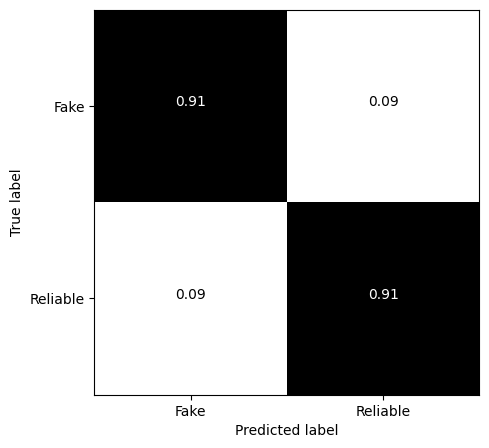
\includegraphics[width=0.7\textwidth]{matrix.png}};
\draw [arrow] (model1) -- (test2);
\draw [arrow] (model2) -- (test3);
\draw [arrow] (model3) -- (test4);

\draw [arrow] (test1) -- (test2);
\draw [arrow] (test2) -- (test3);
\draw [arrow] (test3) -- (test4);
\draw [arrow] (test4) -- (test5);
\end{tikzpicture}
pota
\end{document}
